\documentclass{article}
\usepackage{graphicx} % Load the graphicx package

\begin{document}

\section{Including an Image}

Here’s an example of how to insert an image into your document:

% Basic syntax for including an image
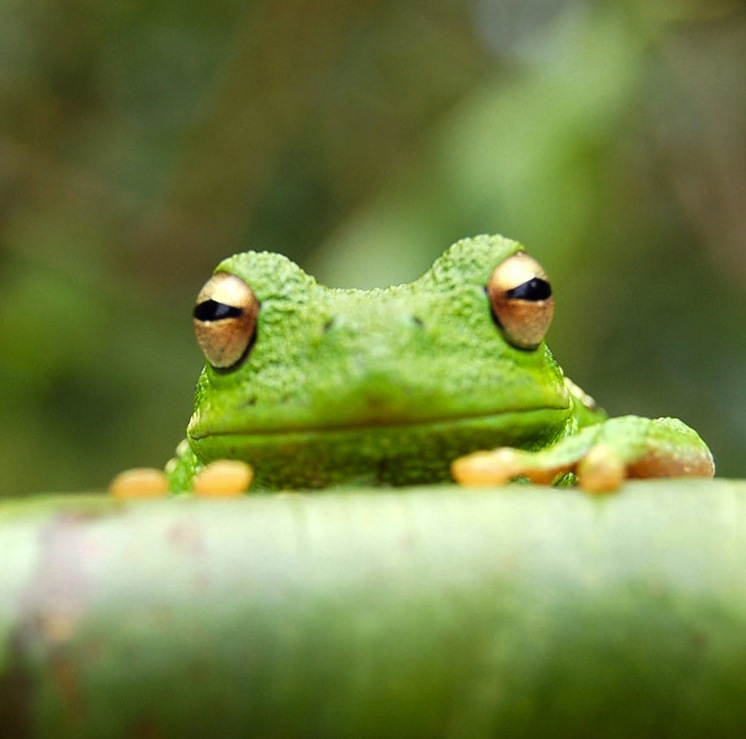
\includegraphics[width=0.5\textwidth]{files/frog.jpg}

% Example: Scaling and rotating an image
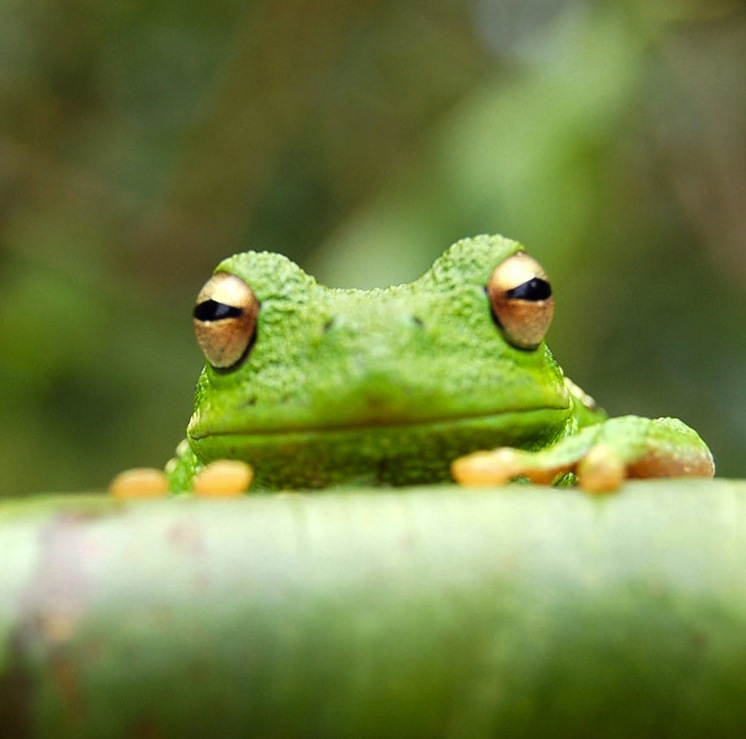
\includegraphics[width=0.5\textwidth, angle=45]{files/frog.jpg}

\section{Image Example}

Below is an example image with various adjustments.

\begin{figure}[ht] % Create a floating figure environment
    \centering % Center the image
    % Include the image with scaling and caption
    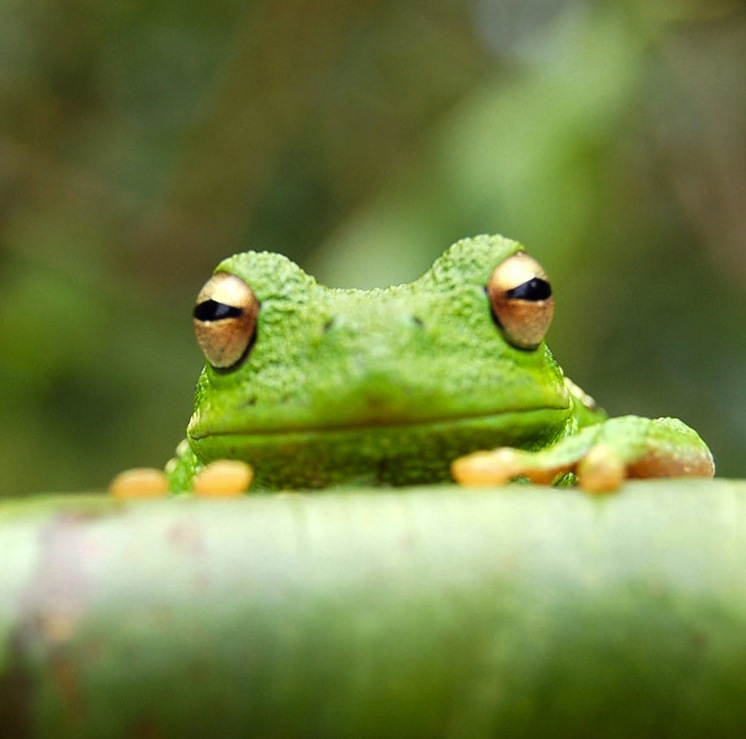
\includegraphics[width=0.5\textwidth, angle=0]{files/frog.jpg}
    \caption{Example image with width scaling}
    \label{fig:example} % Label for referencing
\end{figure}

\end{document}